\documentclass{article}
% load libraries
\usepackage{fontspec}
\usepackage{xeCJK}
\usepackage{mathtools}
\usepackage{graphicx} % Required for inserting images
\usepackage{hyperref}

\title{10-bar Truss Optimization}
\author{DingChun Hsieh}
\date{September 2023}

\begin{document}

\maketitle

\section{Problem}

Figure \ref{fig:Figure 1} shows the structure of the ten bar truss.
Node numbers and element numbers also present in figure \ref{fig:Figure 1}.
\begin{figure}[h]
    \centering
    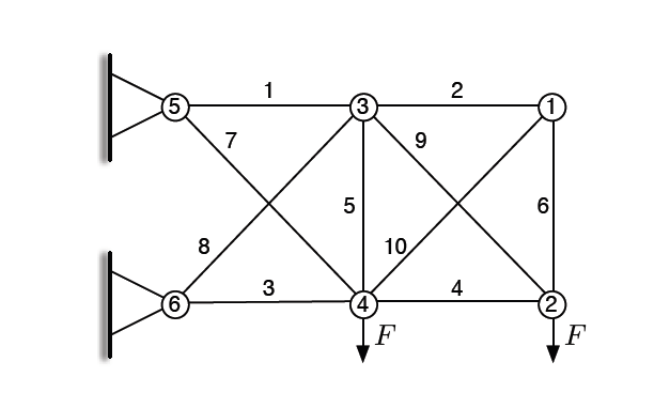
\includegraphics[width=0.5\textwidth]{../images/ten bar.png}
    \caption{Ten bar truss nodes and elements}
    \label{fig:Figure 1}
\end{figure}

Figure \ref{fig:Figure 2} is the optimum formula and constraint for the optimization.   
\begin{figure}[h]
    \centering
    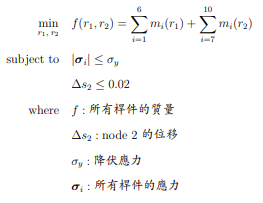
\includegraphics[width=0.5\textwidth]{../images/constraint.png}
    \caption{Optimum formula and constraint}
    \label{fig:Figure 2}
\end{figure}
\clearpage
\textbf{Problem definition}
\begin{itemize}
	\item All the structure under static equilibrium condition.
	\item All the cross-section is circle.
	\item $E = 200 GPa $, $\rho = 7860 kg/ m^3  $, $ \sigma_y = 250 MPa $.
	\item Length of element 1-6 is 9.14 m.
	\item Radius of element 1-6 is $r_1  $, radius of element 7-10 is $r_2$.
	\item 0.001 m $\le$ r $\le$ 0.5 m
	\item Forces apply on node 2, 4 is $ 1.0 \cdot 10^7 N $ downward.
\end{itemize}

\section{Calculation}
Calculation based on Finite Element Truss, using stiffness matrix and input force to calculate element displacement and stress. \\
The calculation is been done with Matlab and posted on \href{https://github.com/dchsieh/Ten-bar-truss-optimization.git}{Git Hub}.

\section{Result}
The result radius of $ r_1 = 0.3000 mm , r_2 = 0.2663 mm. $\\
$ fval = 2.1241e+05 $.


\end{document}
